\documentclass[12pt, twoside]{article}
\usepackage[letterpaper, margin=1in, headsep=0.5in]{geometry}
\usepackage[english]{babel}
\usepackage[utf8]{inputenc}
\usepackage{amsmath}
\usepackage{amsfonts}
\usepackage{amssymb}
\usepackage{tikz}
\usetikzlibrary{quotes, angles}
\usepackage{graphicx}
%\usepackage{pgfplots}
%\pgfplotsset{width=10cm,compat=1.9}
%\usepgfplotslibrary{statistics}
%\usepackage{pgfplotstable}
%\usepackage{tkz-fct}
%\usepackage{venndiagram}
\usepackage{enumitem}
\usepackage{multicol}


\usepackage{fancyhdr}
\pagestyle{fancy}
\fancyhf{}
\fancyhead[LE]{\thepage}
\fancyhead[RO]{\thepage \\Name: \hspace{4cm} \,\\}
\fancyhead[LO]{BECA / Dr. Huson / Geometry 10th Grade\\* Unit 9: Congruence transformations \\ 28 February 2020}

\renewcommand{\headrulewidth}{0pt}

\begin{document}
\subsubsection*{9.5b Exam: Rigid motions, translation, reflection, rotation (No Calculator)}
  \begin{enumerate}

  \item Slide $\triangle ABC$ to the left four and up five. Label the image $\triangle A'B'C'$.
    \begin{center}
        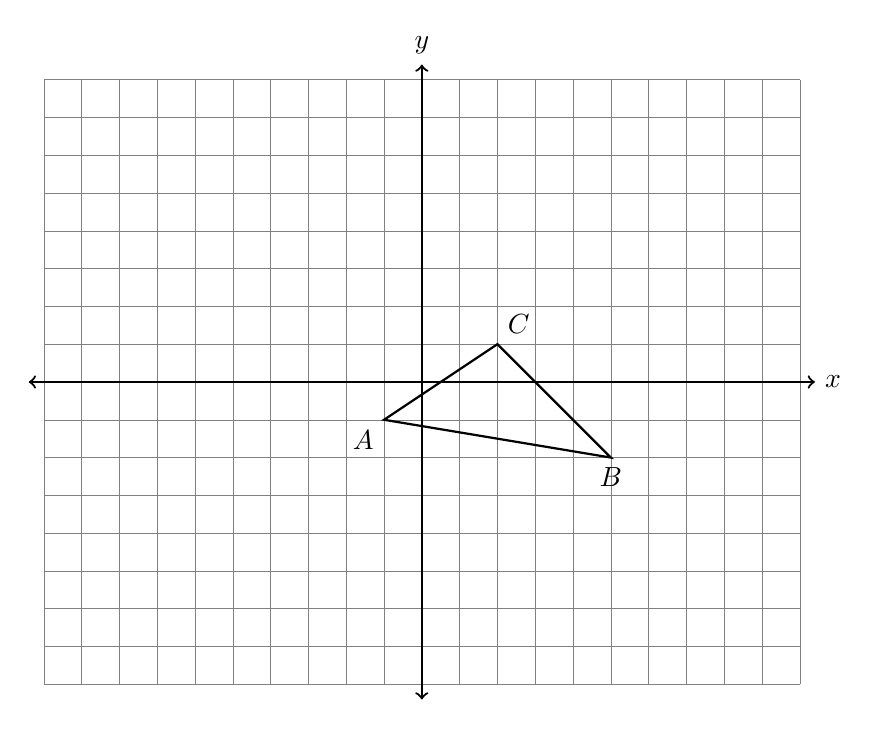
\begin{tikzpicture}[scale=.48]
        \draw [help lines] (-10,-8) grid (10,8);
        \draw [thick, <->] (-10.4,0) -- (10.4,0) node [right] {$x$};
        \draw [thick, <->] (0,-8.4)--(0,8.4) node [above] {$y$};  
        \draw [thick]
          (-1,-1) node[below left] {$A$}--
          (5,-2) node[below] {$B$}--
          (2,1) node[above right] {$C$}--cycle;  
      \end{tikzpicture}
    \end{center}

  \item Apply the translation $(x,y) \rightarrow (x-3,y+5)$ to the point $P(-2,-5)$. \vspace{3cm}
  
  \item On the axes below, graph the point $N(-3,2)$ and its image, $N'$, after a reflection across the $x$-axis. Mark $N'$ and write it down as a coordinate pair.
    \begin{center}
      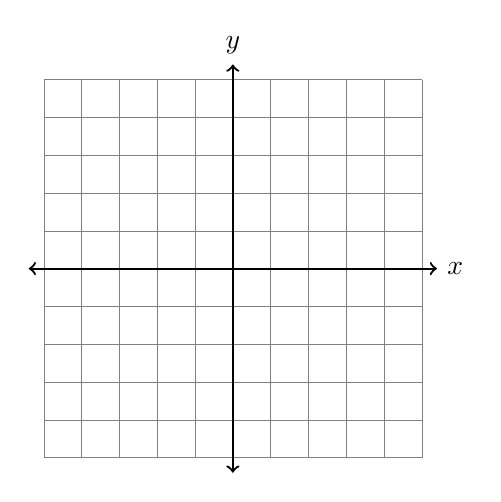
\begin{tikzpicture}[scale=.48]
      \draw [help lines] (-5,-5) grid (5,5);
      \draw [thick, <->] (-5.4,0) -- (5.4,0) node [right] {$x$};
      \draw [thick, <->] (0,-5.4)--(0,5.4) node [above] {$y$};   
    \end{tikzpicture}
  \end{center}

\newpage
  \item Identify the transformation that maps $\triangle ABC$ onto its image $\triangle A'B'C'$.
  \begin{flushright}
      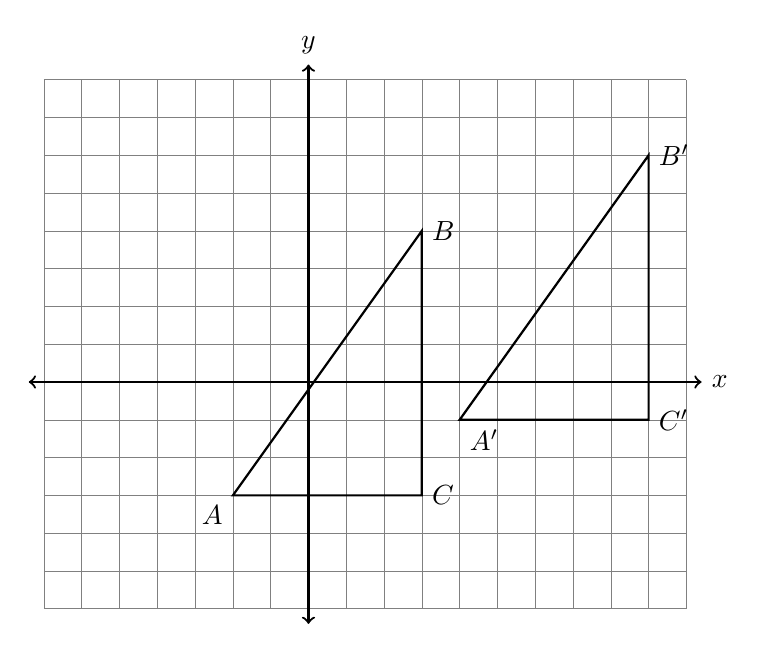
\begin{tikzpicture}[scale=.48]
      \draw [help lines] (-7,-6) grid (10,8);
      \draw [thick, <->] (-7.4,0) -- (10.4,0) node [right] {$x$};
      \draw [thick, <->] (0,-6.4)--(0,8.4) node [above] {$y$};  
      \draw [thick]
        (-2,-3) node[below left] {$A$}--
        (3,4) node[right] {$B$}--
        (3,-3) node[right] {$C$}--cycle;  
      \draw [thick]
        (4,-1) node[below right] {$A'$}--
        (9,6) node[right] {$B'$}--
        (9,-1) node[right] {$C'$}--cycle;   \end{tikzpicture}
  \end{flushright}

  \item State the translation that would map $Q(4,3)$ onto $Q'(-1,-3)$. \vspace{2cm}
  
  \item On the set of axes below, $\triangle ABC \cong \triangle STU$. \\[0.5cm]
  Describe the rigid motion that maps $\triangle ABC$ onto $\triangle STU$.
  \begin{flushright}
      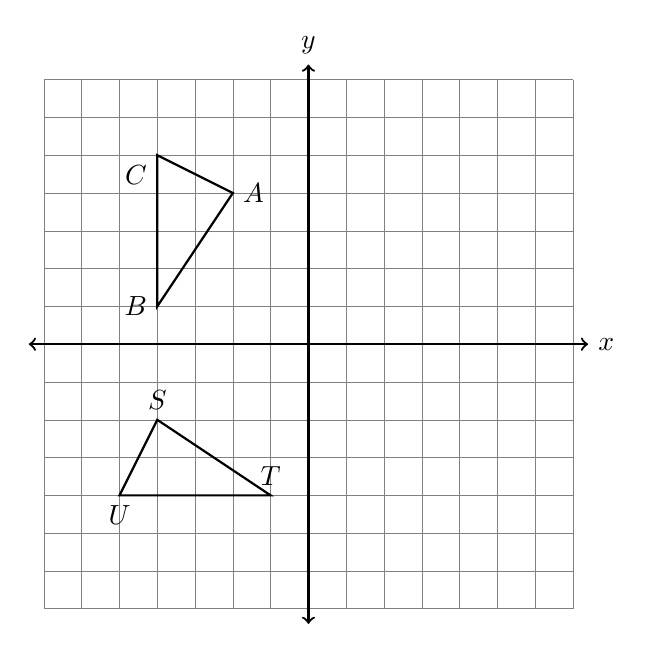
\begin{tikzpicture}[scale=.48]
      \draw [help lines] (-7,-7) grid (7,7);
      \draw [thick, <->] (-7.4,0) -- (7.4,0) node [right] {$x$};
      \draw [thick, <->] (0,-7.4)--(0,7.4) node [above] {$y$};  
      \draw [thick]
        (-2,4) node[right] {$A$}--
        (-4,1) node[left] {$B$}--
        (-4,5) node[below left] {$C$}--cycle;
      \draw [thick]
      (-4,-2) node[above] {$S$}--
      (-1,-4) node[above] {$T$}--
      (-5,-4) node[below] {$U$}--cycle;
    \end{tikzpicture}
  \end{flushright}

\newpage
  \item Triangle $A'B'C'$ is the image of triangle $ABC$ after a translation of 2 units to the right and 3 units up. Is triangle $ABC$ congruent to $A'B'C'$? Explain why. \vspace{3cm}

  \item Rotate $\triangle JKL$ $90^\circ$ counterclockwise around the origin on the axes below, labeling the image $\triangle J'K'L'$.
  \begin{center}
      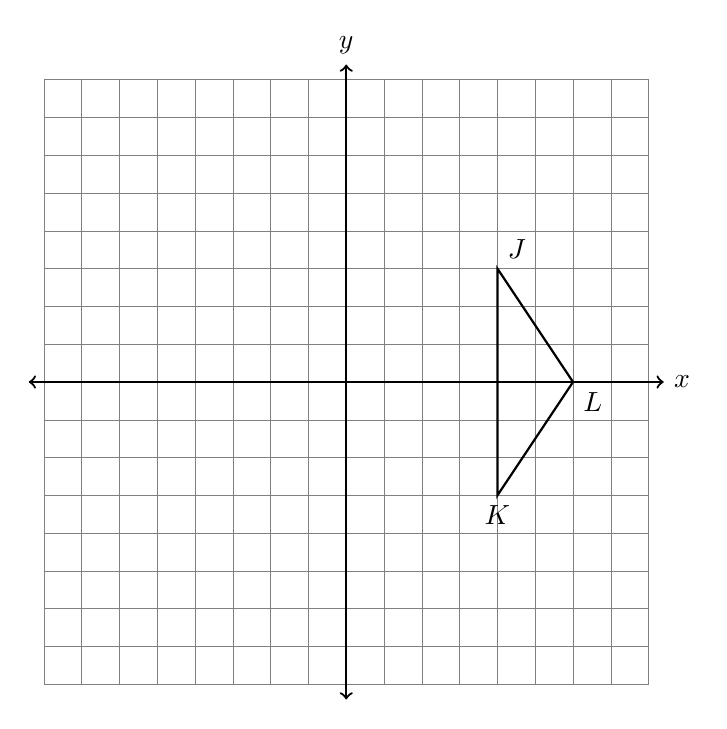
\begin{tikzpicture}[scale=.48]
      \draw [help lines] (-8,-8) grid (8,8);
      \draw [thick, <->] (-8.4,0) -- (8.4,0) node [right] {$x$};
      \draw [thick, <->] (0,-8.4)--(0,8.4) node [above] {$y$};  
      \draw [thick]
        (4,3) node[above right] {$J$}--
        (4,-3) node[below] {$K$}--
        (6,0) node[below right] {$L$}--cycle;  
    \end{tikzpicture}
  \end{center}
  

  \item Draw the line of reflection that would map $\triangle ABC$ onto $\triangle A'B'C'$.
  \begin{center}
      \begin{tikzpicture}[rotate=-100]
      %\draw [help lines] (-7,-2) grid (7,6);
      %\draw [thick, <->] (-7.4,0) -- (7.4,0) node [right] {$x$};
      %\draw [thick, <->] (0,-2.4)--(0,6.4) node [above] {$y$};  
      \draw [thick]
        (0,2) node[left] {$A$}--
        (3,4) node[right] {$B$}--
        (-2,3) node[left] {$C$}--cycle;
      \draw [thick]
      (2,0) node[above] {$A'$}--
      (4,3) node[below left] {$B'$}--
      (3,-2) node[left] {$C'$}--cycle;
    \end{tikzpicture}
  \end{center}

\newpage
\item On the axes below, plot the point $A(-4,-1)$ and its image, $A'$, after the translation $(x,y) \rightarrow (x+6,y-3)$. Label the image as a coordinate pair.
    \begin{center}
      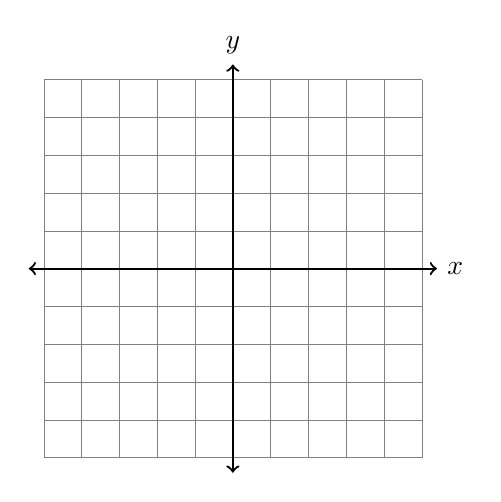
\begin{tikzpicture}[scale=.48]
      \draw [help lines] (-5,-5) grid (5,5);
      \draw [thick, <->] (-5.4,0) -- (5.4,0) node [right] {$x$};
      \draw [thick, <->] (0,-5.4)--(0,5.4) node [above] {$y$};   
    \end{tikzpicture}
  \end{center}

  \item The image of triangle $ABC$ after a translation is $\triangle A'B'C'$. Is the area of the triangle greater, smaller, or the same after the translation? Justify your answer. \vspace{3cm}
  
  \item Determine and state the transformation mapping $\triangle PQR$ onto $\triangle STU$.
  \begin{flushright}
      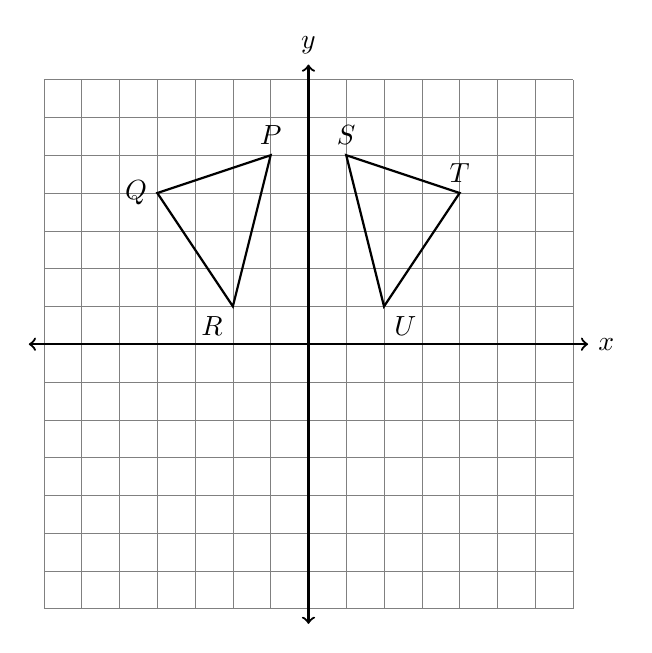
\begin{tikzpicture}[scale=.48]
      \draw [help lines] (-7,-7) grid (7,7);
      \draw [thick, <->] (-7.4,0) -- (7.4,0) node [right] {$x$};
      \draw [thick, <->] (0,-7.4)--(0,7.4) node [above] {$y$};  
      \draw [thick]
        (-1,5) node[above] {$P$}--
        (-4,4) node[left] {$Q$}--
        (-2,1) node[below left] {$R$}--cycle;
      \draw [thick]
      (1,5) node[above] {$S$}--
      (4,4) node[above] {$T$}--
      (2,1) node[below right] {$U$}--cycle;
    \end{tikzpicture}
  \end{flushright}

\newpage
  \item State the translation that would map $C(-4,0)$ onto $C'(3,-3)$. (the use of the grid below is optional)
    \begin{center}
      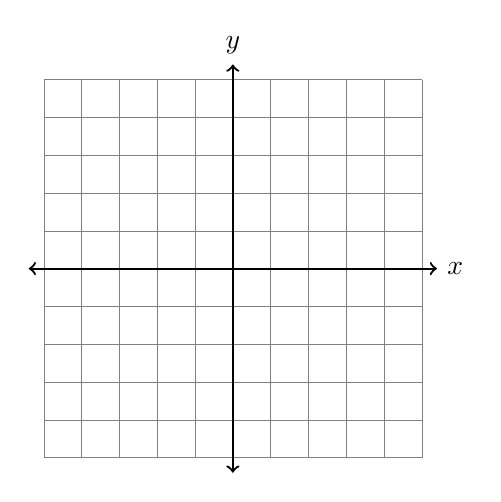
\begin{tikzpicture}[scale=.48]
      \draw [help lines] (-5,-5) grid (5,5);
      \draw [thick, <->] (-5.4,0) -- (5.4,0) node [right] {$x$};
      \draw [thick, <->] (0,-5.4)--(0,5.4) node [above] {$y$};   
    \end{tikzpicture}
  \end{center}

  \item Two transformations have been applied to a triangle in the diagram below, \\$\triangle ABC \rightarrow \triangle A'B'C' \rightarrow \triangle A''B''C''$. Fully characterize each transformation.
  \begin{flushright}
      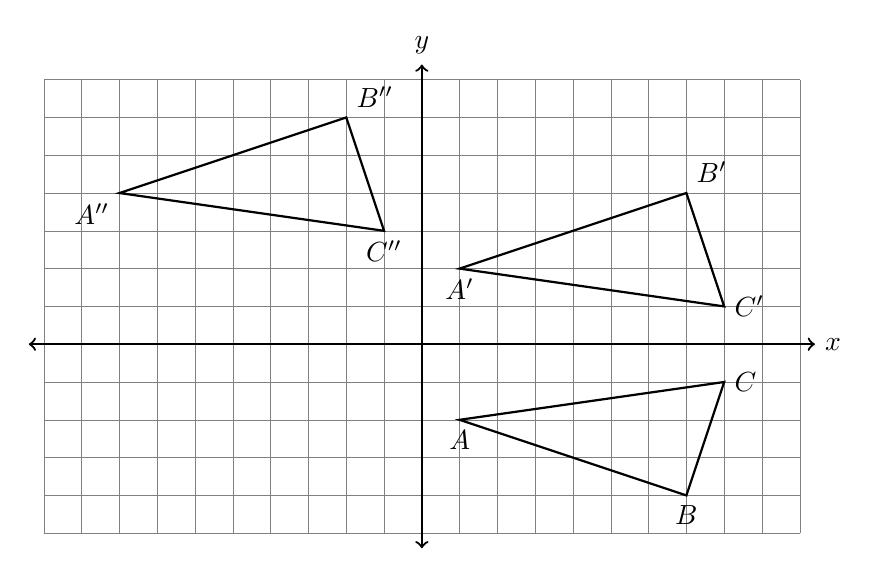
\begin{tikzpicture}[scale=.48]
      \draw [help lines] (-10,-5) grid (10,7);
      \draw [thick, <->] (-10.4,0) -- (10.4,0) node [right] {$x$};
      \draw [thick, <->] (0,-5.4)--(0,7.4) node [above] {$y$};  
      \draw [thick]
        (-8,4) node[below left] {$A''$}--
        (-2,6) node[above right] {$B''$}--
        (-1,3) node[below] {$C''$}--cycle;
      \draw [thick]
        (1,2) node[below] {$A'$}--
        (7,4) node[above right] {$B'$}--
        (8,1) node[right] {$C'$}--cycle;  
        \draw [thick]
        (1,-2) node[below] {$A$}--
        (7,-4) node[below] {$B$}--
        (8,-1) node[right] {$C$}--cycle;
    \end{tikzpicture}
  \end{flushright}

  \item What are the coordinates of the image of $B(2,5)$ after a reflection across the $x$-axis?  \vspace{0.5cm}
    \begin{multicols}{2}
      \begin{enumerate}
      \item $(-2,5)$
      \item $(5,2)$
      \item $(2,-5)$
      \item $(-5,-2)$
    \end{enumerate}
    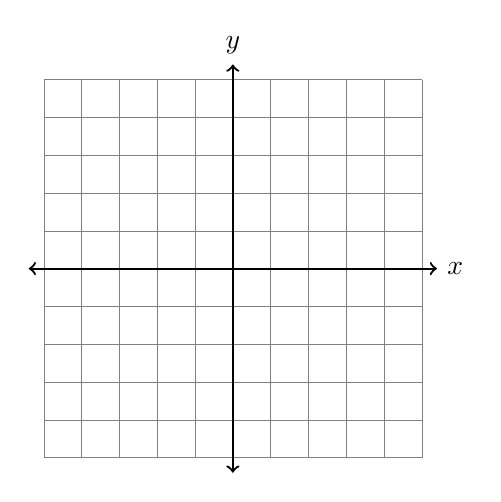
\begin{tikzpicture}[scale=.48]
      \draw [help lines] (-5,-5) grid (5,5);
      \draw [thick, <->] (-5.4,0) -- (5.4,0) node [right] {$x$};
      \draw [thick, <->] (0,-5.4)--(0,5.4) node [above] {$y$};   
    \end{tikzpicture}
  \end{multicols}

\newpage
  \item Which of the following would map $\triangle CAT \rightarrow \triangle C'A'T'$?  \vspace{0.5cm}
    \begin{multicols}{2}
      \begin{itemize}
        \item[T \quad F \quad] Reflected across the $y$-axis
        \item[T \quad F \quad] Translated six to the left, down zero
        \item[T \quad F \quad] Reflected across the $y$-axis, then slid to the left two
        \item[T \quad F \quad] $(x,y) \rightarrow (x-6, y+0)$
        \item[T \quad F \quad] Rotated $90^\circ$ counterclockwise around the origin
        \item[T \quad F \quad] Reflected across the line $x=-1$
      \end{itemize}
    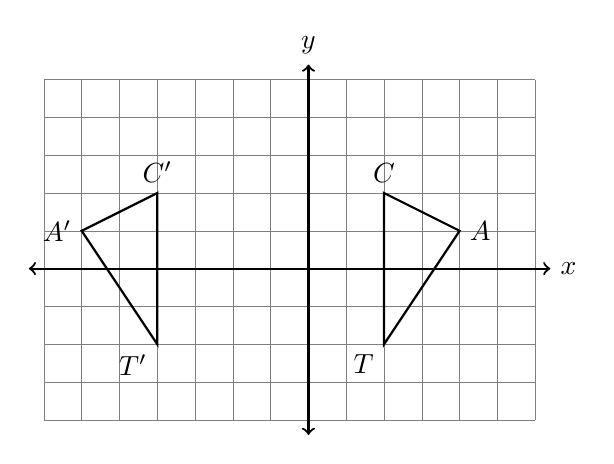
\begin{tikzpicture}[scale=.48]
      \draw [help lines] (-7,-4) grid (6,5);
      \draw [thick, <->] (-7.4,0) -- (6.4,0) node [right] {$x$};
      \draw [thick, <->] (0,-4.4)--(0,5.4) node [above] {$y$};  
      \draw [thick]
      (2,2) node[above] {$C$}--
      (4,1) node[right] {$A$}--
      (2,-2) node[below left] {$T$}--cycle;
      \draw [thick]
      (-4,2) node[above] {$C'$}--
      (-6,1) node[left] {$A'$}--
      (-4,-2) node[below left] {$T'$}--cycle;
    \end{tikzpicture}
  \end{multicols}
  
  \item First reflect the trapezoid $BECA$ across the $x$-axis, then move it down 1 and right 7. Label the images $B'E'C'A'$ and $B''E''C''A''$.
    \begin{center}
        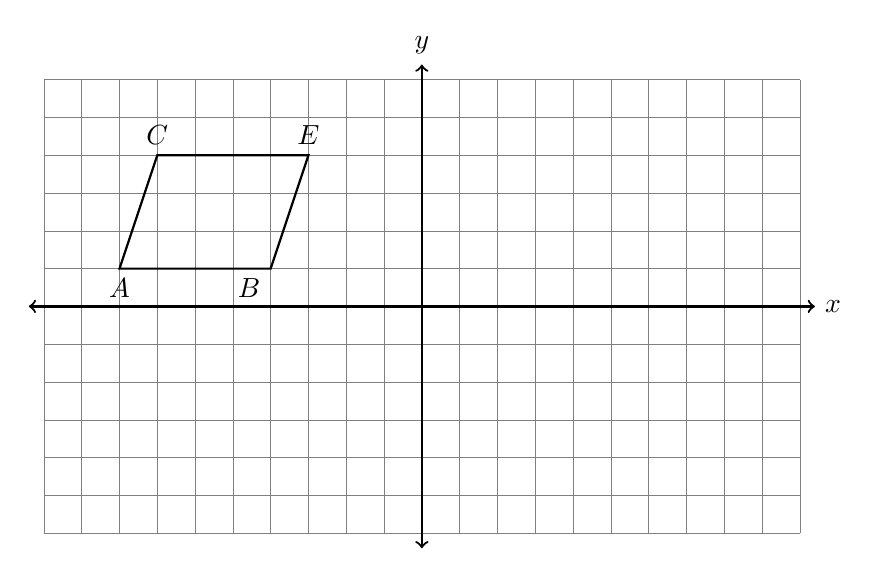
\begin{tikzpicture}[scale=.48]
        \draw [help lines] (-10,-6) grid (10,6);
        \draw [thick, <->] (-10.4,0) -- (10.4,0) node [right] {$x$};
        \draw [thick, <->] (0,-6.4)--(0,6.4) node [above] {$y$};  
        \draw [thick]
          (-4,1) node[below left] {$B$}--
          (-3,4) node[above] {$E$}--
          (-7,4) node[above] {$C$}--
          (-8,1) node[below] {$A$}--cycle;  
      \end{tikzpicture}
    \end{center}

    \item Draw the line of reflection for quadrilaterals in the diagram below.
    \begin{center}
    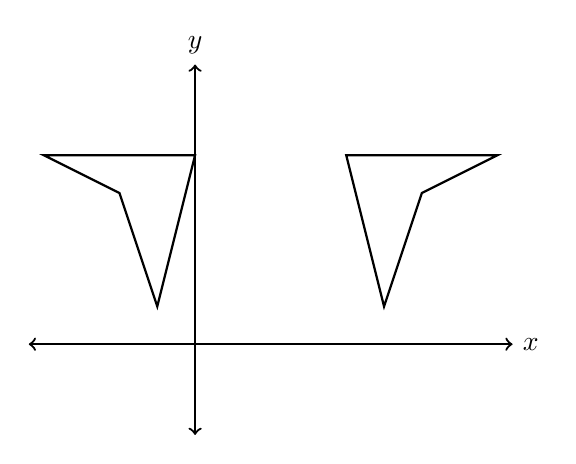
\begin{tikzpicture}[scale=.48]
      %\draw [help lines] (-10,-7) grid (10,7);
      \draw [thick, <->] (-4.4,0) -- (8.4,0) node [right] {$x$};
      \draw [thick, <->] (0,-2.4)--(0,7.4) node [above] {$y$};  
      \draw [thick](5,1)--(6,4)--(8,5)--(4,5)--cycle;  
      \draw [thick](-1,1)--(-2,4)--(-4,5)--(0,5)--cycle;
    \end{tikzpicture}
  \end{center}

\newpage
  \item The quadrilateral $ROCK$ undergoes rigid motions, shown below. Describe the sequence of transformations applied.
  \begin{flushright}
      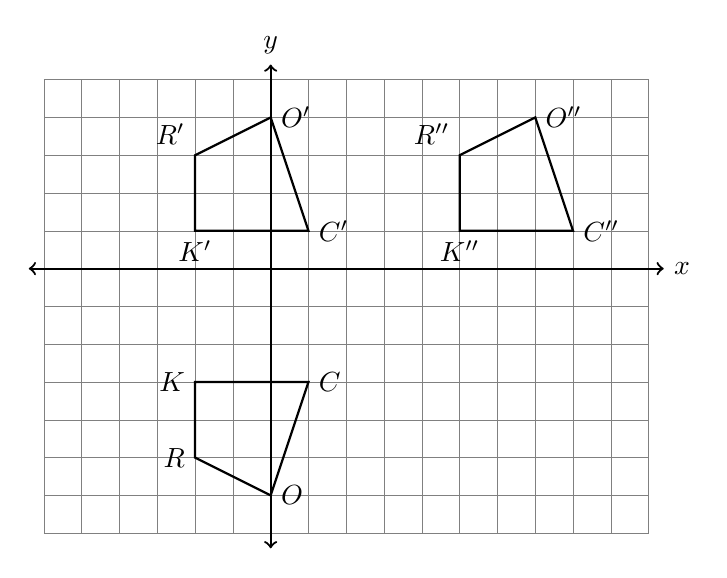
\begin{tikzpicture}[scale=.48]
      \draw [help lines] (-6,-7) grid (10,5);
      \draw [thick, <->] (-6.4,0) -- (10.4,0) node [right] {$x$};
      \draw [thick, <->] (0,-7.4)--(0,5.4) node [above] {$y$};  
      \draw [thick]
        (5,1) node[below] {$K''$}--
        (5,3) node[above left] {$R''$}--
        (7,4) node[right] {$O''$}--
        (8,1) node[right] {$C''$}--cycle;
      \draw [thick]
        (-2,1) node[below] {$K'$}--
        (-2,3) node[above left] {$R'$}--
        (0,4) node[right] {$O'$}--
        (1,1) node[right] {$C'$}--cycle;  
      \draw [thick]
      (-2,-3) node[left] {$K$}--
      (-2,-5) node[left] {$R$}--
      (0,-6) node[right] {$O$}--
      (1,-3) node[right] {$C$}--cycle;
    \end{tikzpicture}
  \end{flushright}

  \item The quadrilateral $MATH$ is mapped to $M'A'T'H'$ by a rigid motion. What transformation a been applied?  \vspace{0.5cm}
  \begin{multicols}{2}
    \begin{enumerate}
      \item Dilation
      \item Reflection
      \item Rotation
      \item Translation
    \end{enumerate}
    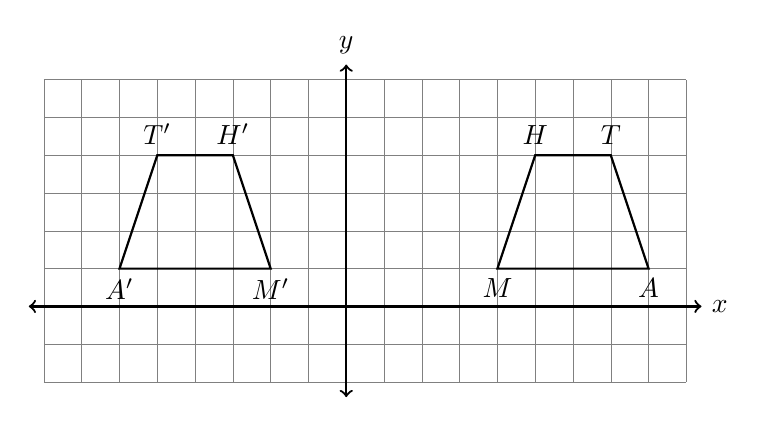
\begin{tikzpicture}[scale=.48]
      \draw [help lines] (-8,-2) grid (9,6);
      \draw [thick, <->] (-8.4,0) -- (9.4,0) node [right] {$x$};
      \draw [thick, <->] (0,-2.4)--(0,6.4) node [above] {$y$};  
      \draw [thick]
        (4,1) node[below] {$M$}--
        (8,1) node[below] {$A$}--
        (7,4) node[above] {$T$}--
        (5,4) node[above] {$H$}--cycle;
      \draw [thick]
        (-2,1) node[below] {$M'$}--
        (-6,1) node[below] {$A'$}--
        (-5,4) node[above] {$T'$}--
        (-3,4) node[above] {$H'$}--cycle; 
    \end{tikzpicture}
  \end{multicols}

  \item What are the coordinates of the image of $C(4,0)$ after a rotation of $90^\circ$ counterclockwise around the origin? \vspace{0.5cm}
    \begin{multicols}{2}
      \begin{enumerate}
        \item $(4,4)$
        \item $(0,4)$
        \item $(-4,0)$
        \item $(0,-4)$
      \end{enumerate}
      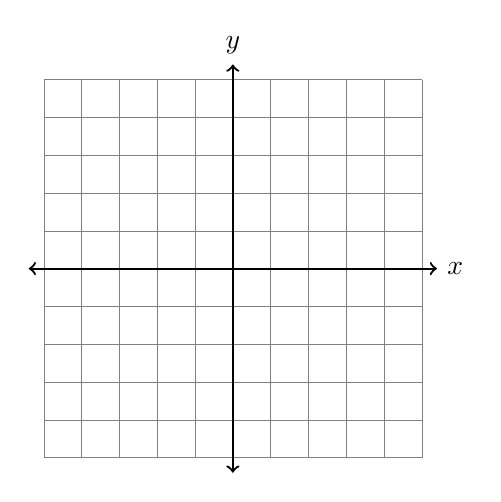
\begin{tikzpicture}[scale=.48]
        \draw [help lines] (-5,-5) grid (5,5);
        \draw [thick, <->] (-5.4,0) -- (5.4,0) node [right] {$x$};
        \draw [thick, <->] (0,-5.4)--(0,5.4) node [above] {$y$};   
      \end{tikzpicture}
    \end{multicols}

\newpage
  \item Given $\triangle WIN \cong \triangle W'I'N'$. Describe the rigid motion mapping $\triangle WIN \rightarrow \triangle W'I'N'$.
  \begin{flushright}
    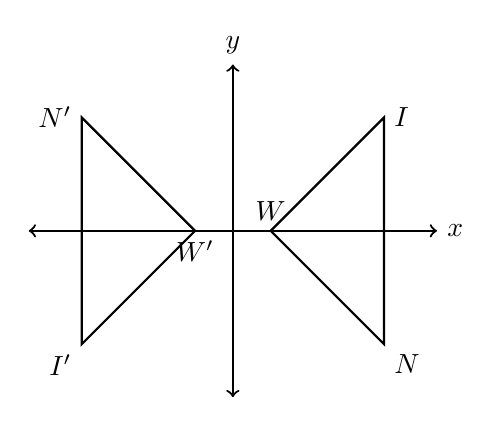
\begin{tikzpicture}[scale=.48]
      %\draw [help lines] (-10,-7) grid (10,7);
      \draw [thick, <->] (-5.4,0) -- (5.4,0) node [right] {$x$};
      \draw [thick, <->] (0,-4.4)--(0,4.4) node [above] {$y$};  
      \draw [thick]
      (1,0) node[above] {$W$}--
      (4,3) node[right] {$I$}--
      (4,-3) node[below right] {$N$}--cycle;
      \draw [thick]
      (-1,0) node[below] {$W'$}--
      (-4,3) node[left] {$N'$}--
      (-4,-3) node[below left] {$I'$}--cycle;
    \end{tikzpicture}
  \end{flushright}

  \item Determine and state the sequence of transfromations applied to map $BECA$ to $B''E''C''A''$.
  \begin{flushright}
      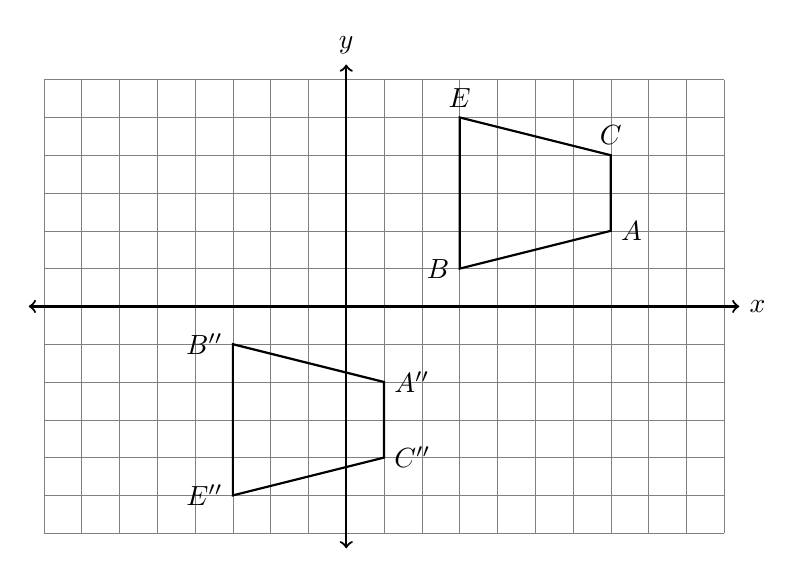
\begin{tikzpicture}[scale=.48]
      \draw [help lines] (-8,-6) grid (10,6);
      \draw [thick, <->] (-8.4,0) -- (10.4,0) node [right] {$x$};
      \draw [thick, <->] (0,-6.4)--(0,6.4) node [above] {$y$};  
      \draw [thick]
        (3,1) node[left] {$B$}--
        (3,5) node[above] {$E$}--
        (7,4) node[above] {$C$}--
        (7,2) node[right] {$A$}--cycle;
      \draw [thick]
        (-3,-1) node[left] {$B''$}--
        (-3,-5) node[left] {$E''$}--
        (1,-4) node[right] {$C''$}--
        (1,-2) node[right] {$A''$}--cycle; 
    \end{tikzpicture}
  \end{flushright}

  \item Determine and state the transformation mapping $\triangle NOP$ onto $\triangle QRP$. 
    \begin{flushright}
        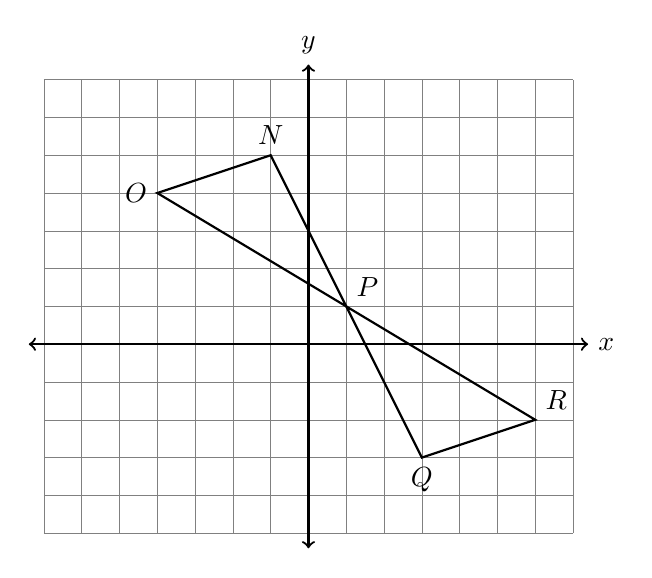
\begin{tikzpicture}[scale=.48]
        \draw [help lines] (-7,-5) grid (7,7);
        \draw [thick, <->] (-7.4,0) -- (7.4,0) node [right] {$x$};
        \draw [thick, <->] (0,-5.4)--(0,7.4) node [above] {$y$};  
        \draw [thick]
          (-1,5) node[above] {$N$}--
          (-4,4) node[left] {$O$}--
          (1,1) --cycle;
        \draw [thick]
        (3,-3) node[below] {$Q$}--
        (6,-2) node[above right] {$R$}--
        (1,1) node[above right] {$P$}--cycle;
      \end{tikzpicture}
    \end{flushright}

\end{enumerate}
\end{document}

